\section{Python Basics}

	In order to write programs to perform cryptography, we will need to be able to manipulate words and sentences, which in programming we call \textit{strings}.
	
	We'll start with some basic Python programs, which will teach us everything we need in order to pull words and sentences apart.
	
	\begin{figure}[h]
		\centering
		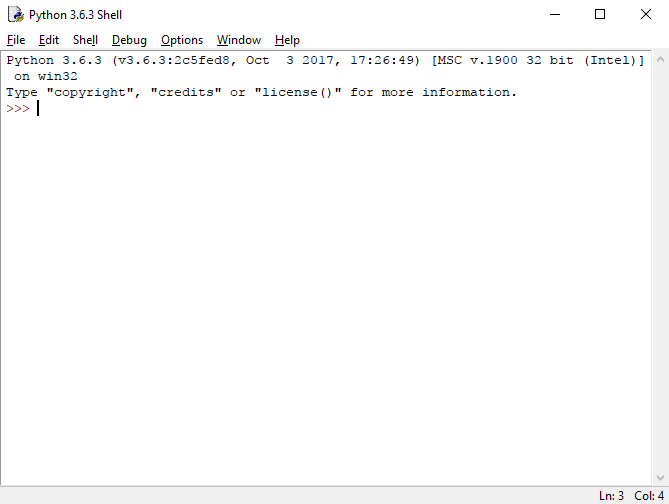
\includegraphics[width=0.8\linewidth]{McrRaspJam/016_Ciphers/1_python/idle}
		\caption{The IDLE \textit{shell} window}
		\label{fig:idle}
	\end{figure}
	
	Go to the main menu on your Raspberry Pi desktop and \textbf{open} the application titled \textit{Python 3 (IDLE)}.
	
	After a few seconds, IDLE will open to the \textit{Python Shell}. In this window, go to \textbf{File $\rightarrow$ New File}, which will open an empty window where we can write our programs.
	
	\subsection*{Hello, World!}
		
		In your empty window, \textbf{copy} the following program:
		
		\lstinputlisting[style=Python, title=helloworld.py]{McrRaspJam/016_Ciphers/1_python/helloworld.py}
		
		then, select \textbf{Run $\rightarrow$ Run Module} at the top of the window.
		
		After saving, your program will run and ``Hello, World!'' should appear in the shell window in blue.
		
	\subsection*{Inputting text}
	
		The next thing we'll need for our cipher programs is to enter text when our program runs. \textbf{Modify} your code to add the following command.
		
		\lstinputlisting[style=Python]{McrRaspJam/016_Ciphers/1_python/input.py}
		
		\textbf{Run} your program again. This time you will be asked to enter text into the shell window, and when you press enter it will be repeated back to you.
		
		\begin{aside}[Variables]
			When we store data (like text or numbers) in our programs, we store them as \textit{variables}.
			
			A variable has a \textit{label}---what the variable is called---and a \textit{value}---the data we wish to store in it.
			
			When we `set' a variable, we call this an \textit{assignment}, signified by the \texttt{=} sign.
		\end{aside}
	
	\subsection*{Lists}
	
		It is often useful to store several pieces of data in a single variable. A common way of doing this in Python is to use a list.
		
		\textbf{Open} a new file by selecting \textbf{File $\rightarrow$ New File}, then write the following program in the new window:
		
		\lstinputlisting[style=Python, title=list.py, breaklines=true]{McrRaspJam/016_Ciphers/1_python/list.py}
		
		Before you run your program, have a guess what will be printed out when you run the program. Run your program, then see whether what was printed matched what you thought it would be.
		
		\textit{extra challenge:} How can we fix the word spacing in the printed text?
		
		\begin{aside}[Lists]
			When we add \textit{elements} of data to a list, they are given the next available \textit{index} number.
			
			\vspace{4pt}
			\begin{tabular}{c|c}
				0 & Vanilla \\ 
				1 & Strawberry \\ 
				2 & Chocolate \\ 
				3 & Raspberry Ripple
			\end{tabular} 
			\vspace{4pt}
						
			To access a single element from a list, we use square brackets, as we have done in our program above.
		\end{aside}
	
	\subsection*{Strings are Lists}
	
		When we write our cipher programs, we'll need to look at single letters from the sentences we input. In python, a text \texttt{string} is actually a list of single \texttt{characters}.
		
		This means that we can access a string just like a list. Return to your hello world program, and \textbf{modify} the print statement as follows.
	
		\textbf{\lstinputlisting[style=Python, title=helloworld.py]{McrRaspJam/016_Ciphers/1_python/inputlist.py}}
		
		Now, when you run your program, only the first letter of whatever you typed in will be printed out.
		
		Next, we'll try printing out each letter one-by-one, which we can do using a \textit{loop}.
		
		\textbf{\lstinputlisting[style=Python, title=helloworld.py]{McrRaspJam/016_Ciphers/1_python/inputlist2.py}}
		
		The \texttt{for} loop we used repeats once for each element in the list that we provide it, in this case each letter in our string.
		
		\textbf{Run} your program, and this time your text should be printed one character at a time, each on its own line.
		